\section{System}
\label{sec:sys}

Our \ql system implementation builds on Apache Spark with GraphX.  We
selected Spark because it is a popular open-source system, and because
of its in-memory processing approach.  All \tg operations are
available through the public API of the \ql library, and may be used
like any other library in an Apache Spark application.\eat{  \insql{TGraph}
is the main abstract class that all physical representations extend.
An excerpt of the API, where VD is the vertex attribute and ED is the
edge attribute type:}

\eat{\begin{lstlisting}
def slice(bound: Interval): TGraph[VD, ED]
def aggregate(window: WindowSpecification, vquant: Quantification, equant: Quantification, vAggFunc: (VD, VD) => VD, eAggFunc: (ED, ED) => ED)(vgroupby: (VertexId, VD) => VertexId): TGraph[VD, ED]
def union(other: TGraph[VD, ED]): TGraph[Set[VD], Set[ED]]
\end{lstlisting}}

\subsection{Physical Representations}
\label{sec:sys:datastructs}

We considered four in-memory \tg representations that differ both in
compactness and in the kind of locality they prioritize. With {\em
  structural locality}, neighboring vertices (resp. edges) of the same
representative graph are laid out together, while with {\em temporal
  locality}, consecutive states of the same vertex (resp. edge) are
laid out together~\cite{DBLP:journals/tos/MiaoHLWYZPCC15}.  We now
describe each representation.\eat{ VertexEdge (VE) is a direct
  translation of the \ve model of Definition~\ref{def:tg_ve} and the
  most compact representation.  While VE does not necessitate a
  particular order of tuples on disk, we opt for a physical layout in
  which all tuples corresponding to the same vertex (resp. edge) are
  laid out consecutively, and so VE preserves temporal localilty.
  RepresentativeGraphs (RG) directly implements the data structure of
  Definition~\ref{def:tg_abstract}, storing each representative graph
  explicitly, and so naturally preserves structural locality, but
  temporal locality is lost.  OneGraph (OG) stores all vertices and
  edges of an evolving graph once, in a single data structure.  This
  representation emphasizes temporal locality, while also preserving
  structural locality.  HybridGraph (HG) trades compactness for better
  structural locality, by aggregating together several consecutive
  RGs, and computing a OneGraph for each RG group.  Details of our
  implementation of the four representations are given below.}

\eat{\reminder{Support experimentally or remove / rephrase: We can convert
  from one representation to any other at small or no cost, so it is
  useful to think of them as access methods in the context of
  individual operations.}}

\eat{
\begin{table*}[t]
\centering
\small
\begin{tabular}{ p{1.6cm} | p{3.5cm} | p{3.5cm} | p{3.5cm} | p{3.5cm} }
\hline
\multicolumn{1}{l|}{\bfseries Operation} & \multicolumn{1}{c|}{\bfseries VE} & \multicolumn{1}{c|}{\bfseries RG} & \multicolumn{1}{c|}{\bfseries OG} & \multicolumn{1}{c|}{\bfseries HG} \\ \hline
slice & filter V and E; modify periods to be within slice interval & slice sequence of RGs & filter indices in bitsets & slice sequence of OGs and filter indices in remaining OGs \\ \hline
select & filter V ad E; enforce FK constraint & only when predicate not on interval: filter V and E of each RG & N/A & N/A \\ \hline
project & apply projection to each element of defined projection; coalesce & apply projection to each element within each RG; coalesce and recompute & N/A & N/A \\ \hline
aggregate (non-structural) & split each vertex/edge by window; reduce by window key; filter those under quantification threshold; enforce FK constraint & map each RG to windows; group vertices/edges in each window into one RG, filtering by quantification & only structure: for each vertex/edge map indices in bitsets to corresponding windows; filter by quantification threshold; enforce FK constraint & only structure: combine OGs as necessary to group into windows; map indices in bitsets; filter by quantification threshold; enforce FK constraint \\ \hline
aggregate (with structural) & map each vertex to new id; join edges with new vertices to get new id; rest as above & within each window map vertices and edge triplets to new ids; rest as above & N/A & N/A \\ \hline
union & compute combined intervals; split each vertex/edge by new intervals; full outer join & compute combined intervals; combine RGs in corresponding intervals; full outer join & structure only: remap bitsets to new intervals; union vertices/edges from two graphs and reduce by key to combine bitsets & structure only: combine OGs as necessary; rest as in OG \\ \hline
intersection & compute intervals; split each vertex/edge by new interval; inner join & compute intervals; inner join of vertices/edges from corresponding intervals & structure only: like union but with bitset intersection & structure only: like union but with bitset intersection \\ \hline
analytics (pagerank, shortest paths, etc.) & N/A & compute for each RG & compute for all periods simultaneously & compute for all periods within each OG simultaneously \\ 
\hline
\end{tabular}
\caption{Operations.}
\label{tab:operations}
\end{table*}
}

{\bf RepresentativeGraphs (RG)} is a direct implementation of \trg of
Definition~\ref{def:tg_abstract}.  RG is a collection (parallel
sequence) of GraphX graphs, where vertices and edges store the
attribute values for the specific time interval.  This representation
supports all operations of \tg algebra.

While the \rg representation is simple, it is not compact, considering
that in many real-world evolving graphs there is a 80\% or larger
similarity between consecutive
snapshots~\cite{DBLP:journals/tos/MiaoHLWYZPCC15}.  In a distributed
architecture, however, this data structure provides some benefits as
operations on it can be easily parallelized by assigning different
\rgs to different workers, or by partitioning an \rg across workers.

\rg is the most immediate way to implement evolving graphs using Graph
X. Without \ql a user wishing to analyze evolving graphs might
implement and use the \rg approach.  However, as we will show in
Section~\ref{sec:exp}, this would lead to poor performance for most
operations.

\begin{figure}[t!]
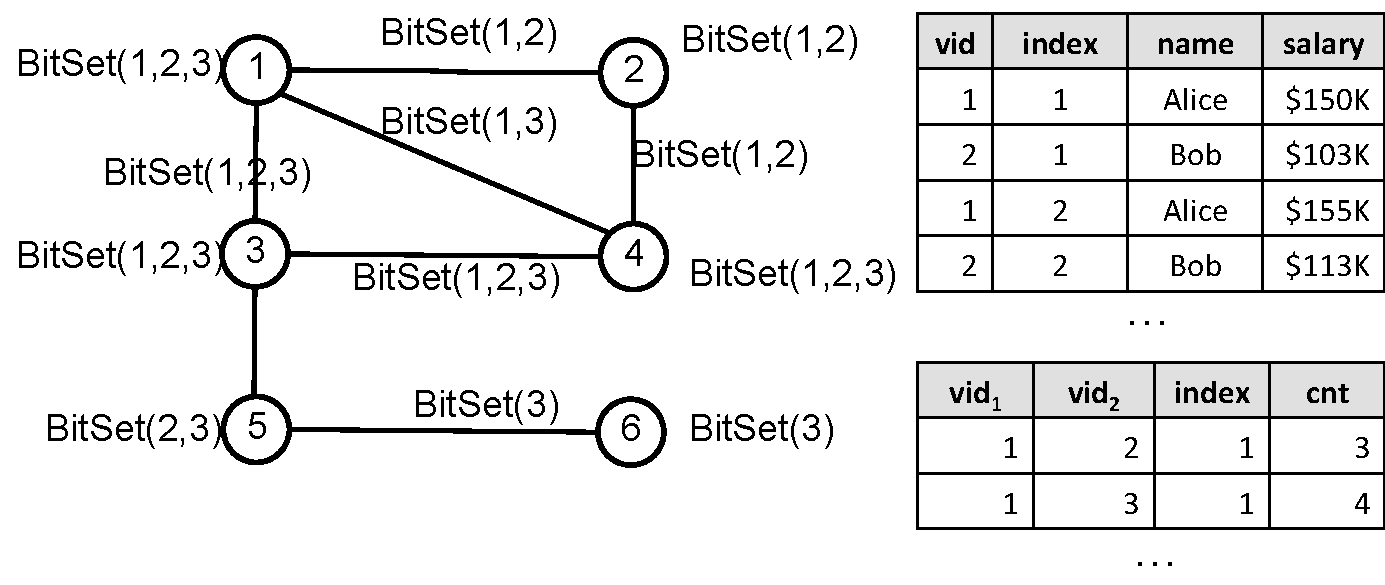
\includegraphics[width=3in]{figs/ogc.pdf}
\caption{\og representation of \insql{T1}.}
\label{fig:ogc}
\end{figure}

{\bf VertexEdge (VE)} is a direct implementation of the \tve model of
Definition~\ref{def:tg}, and is the most compact: one RDD contains
all vertices and another all edges.  Consistently with the GraphX API,
all vertex properties are stored together as a single nested
attribute, as are all edge properties.  While VE does not necessitate
a particular order of tuples on disk, we opt for a physical layout in
which all tuples corresponding to the same vertex (resp. edge) are
laid out consecutively, and so VE preserves temporal localilty.

\eat{ The main advantage of this schema-less attribute representation
  is that it can easily deal with schema evolution and leaves the
  details of attribute processing to the user. } 

The VE representation supports all \tg algebra operations but cannot
support analytics.  This is because an analytic is defined on a
representative graph, which VE does not materialize.  As we will show
in Section~\ref{sec:experiments}, due to compactness this physical
representation is the most efficient for many operations.

{\bf OneGraph (OG)} is the most topologically compact representation,
which stores all vertices {\em and} edges of an evolving graph once,
in a single data structure.  Information about time validity is stored
together with each vertex and edge.  Figure~\ref{fig:ogc} shows the OG
for \tg \insql{T1} from Figure~\ref{fig:tg_rg}.  OG emphasizes
temporal locality, while also preserving structural locality, but
leads to a much denser graph than RG.  This, in turn, makes
parallelizing computation challenging.

An OG is implemented as a single GraphX graph.  To construct an \og
from VE, vertices and edges of \tv and \te relations each are grouped
by key and mapped to bitsets, which in turn encode the presence of a
vertex or edge in each time period associated with some representative
graph of a \tg.  Because \og stored information only about graph
topology, far fewer periods need be represented and computed for \og
than for \rg.  The actual reduction depends on the rate and nature of
graph evolution.

As we will see experimentally in Section~\ref{sec:exp}, \og is often
the best-performing data structure for aggregation, and also has
competitive performance for analytics.  Because of this focus, \og
supports operations only on topology: analytics and
aggregation/union/intersection for graphs with no vertex or edge
attributes.  For completeness, all other operations are supported
through inheritance from an abstract parent, and are carried out on
the VE data structure.

{\bf HybridGraph (HG)} trades compactness of OG for getter structural
locality of RG, by aggregating together several consecutive RGs,
computing a single OG for each RG group, and storing these as a
parallel sequence.  In our current implementation each OG in the
sequence corresponds to the same number of temporally adjacent RGs.

This is the simplest grouping method, and we observed that placing the
same number of RGs into each group often results in unbalanced group
sizes.  This is because evolving graphs commonly exhibit strong
temporal skew, with later RGs being significantly larger than earlier
ones.  We are currently working on more sophisticated grouping
approaches that would lead to better balance, and ultimately to better
performance.  However as we will see experimentally in
Section~\ref{sec:exp}, the current HG implementation already improves
performance compared to OG, in some cases significantly.

Like OG, the HG representation focuses on topology-based analysis, and
so does not represent vertex and edge attributes, only implements
analytics and aggregation/union/intersection, and supports all other
algebraic operations through inheritance from VE.

\subsection{Maintenance Operations}
\label{sec:sys:maint}

\eat{
\begin{table}
\small
\begin{tabular}{ l | p{4cm} | c }
\hline
\multicolumn{1}{l|}{\bfseries Operation} & \multicolumn{1}{c|}{\bfseries Requires Coalesced Input} & \multicolumn{1}{c}{\bfseries Uncoalesces} \\ \hline
slice & no & no \\ \hline
select & only if predicate incl. interval & no \\ \hline
project & no & yes \\ \hline
aggregate & only if structural group by is used and includes interval & yes \\ \hline
union & no & yes \\ \hline
intersection & no & yes \\ \hline
analytics & no & yes \\
\hline
\end{tabular}
\caption{Coalesce analysis.}
\label{tab:coalesce}
\end{table}
}

{\bf Coalescing.}  All algebraic operations, and all sequences of
operations, must output a valid temporally coalesced \tg.  The \ql
system supports both eager and lazy coalescing, with lazy being the
default behavior for multi-operator queries.  Interestingly,
correctness of \tg algebra operations does not depend on whether the
input was coalesced, and so coalescing can be deferred.  To see why
this is so, consider a \insql{slice} operation.  \insql{slice} can be
evaluated on a graph-by-graph or vertex/edge basis.  Let us assume
that there are two consecutive graphs that are the same, i.e. that \sg
is uncoalesced, and that the slice period overlaps with one of these
two graph periods. We can slice the interval of that graph and
coalesce and the result would be the same as if we coalesced first.
\insql{select} operation is orthogonal to time and is applied to each
entity in each time interval.  There is one exception to this rule:
aggregation by change.  When aggregating by change, the input must be
coalesced to compute correct aggregation windows.  If the input is not
coalesced, then there may be two or more consecutive intervals which
should be treated as one but would count separately.

There are several different implementations possible for the coalesce
operation over temporal SQL relations,
see~\cite{DBLP:conf/vldb/BohlenSS96} for detailed analysis.  We use a
partitioning method, where the relation (e.g., \tv, \te, \trg) is
grouped by key, and within each group the tuples are sorted and folded
to produce the corresponding time periods of maximum length.  This
approach involves shuffling between partitions, one of the most
computationally expensive aspects of distributed systems, and thus
lazy coalescing is preferred.\eat{ As with duplicate elimintation, if
  the coalesced output is expected to be significantly reduced in
  size, such as after a project operation on a high volatility
  attribute, performing coalesce eagerly before a time-consuming
  operation, especially analytics, can be advantageous.}

{\bf Foreign key constraint.} \reminder{Yet to read/revise this part.}
The vertex-edge data model includes a foreign key constraint from
edges to vertices.  This constraint is naturally maintained by most
operations while performing operations on V and E independently.  For
\insql{select} and \insql{aggregate} additional steps are required to
insure correctness.  We modify E tuples to enforce the foreign key
constraint by joining on V, using either a broadcast or hash join
depending on the size of V.  Each edge period is then modified to be
the overlap of the periods of source and destination vertices and the
original edge period.  Because this step is computationally expensive,
it is only taken when necessary: when \insql{select} has a predicate
on V and when \insql{aggregate} has a higher level of quantification
for V than for E.  GraphX graphs maintain foreign key constraint
during subgraph operation and we make use of this for all
representations besides VE.

{\bf Partitioning.}  Graph partitioning can have a tremendous impact
on system performance.  A good partitioning strategy needs to (1) be
balanced, assigning an approximately equal number of units to each
partition, and (2) limit the number of cuts across partitions, to
reduce cross-partition communication.  In our experiments we compare
performance with (1) no repartitioning after load, and (2) with
repartitioning using the 2D edge partitioning strategy (E2D).  This
strategy is available in GraphX and was used without modification.  In
E2D, a sparse edge adjacency matrix is partitioned in two dimensions,
guaranteeing a $2 \sqrt{n}$ bound on vertex replication, where $n$ is
the number of partitions. As has been shown
previously~\cite{DBLP:conf/osdi/GonzalezXDCFS14,MoffittTempWeb16}, E2D
provides good performance for Pregel-style analytics.

